\documentclass{article}

%%%%%%%%%%%%%%% LIBRERIAS %%%%%%%%%%%%%%%%%%%%%
\usepackage{amsmath}
\usepackage{titlesec}
\usepackage{titletoc}
\usepackage{graphicx}
\usepackage[spanish,es-tabla]{babel} % 'es-tabla' cambia Cuadro→Tabla
\usepackage{hyperref}                % cargar después de babel
\usepackage{float}
\usepackage{circuitikz}
\usepackage[a4paper, margin=3cm]{geometry}
%%%%%%%%%%%%%%%%%%% VARIABLES %%%%%%%%%%%%%%%%%%%%
\newcommand{\Facultad}{Instituto Tecnológico \\de\\ Buenos Aires} %constantes
\newcommand{\TPn}{Trabajo Práctico N° 1}
\newcommand{\TPtema}{Corriente Continua}
\renewcommand{\thesection}{\arabic{section}}          % 2
\renewcommand{\thesubsection}{\quad \alph{subsection}}   % a
\renewcommand{\thesubsubsection}{\quad \thesubsection.~\roman{subsubsection}} % a. i
\graphicspath{{imagenes&matlab/}} %para que acceda a las fotos en la carpeta directamente


%%%%%%%%%%%%%%%%%% FORMATO TÍTULO Y NUMERACIÓN %%%%%%%%%%%%%%%%%%%
% Numeración de secciones
\renewcommand{\thesection}{\arabic{section}.}          
\renewcommand{\thesubsection}{\thesection\arabic{subsection}}       
\renewcommand{\thesubsubsection}{$\alph{subsubsection})$}

% Numerar hasta subsubsecciones
\setcounter{secnumdepth}{3}

% Formato de títulos
\titleformat{\section}{\Huge\bfseries}{\thesection}{1em}{}
\titleformat{\subsection}{\LARGE\bfseries}{\thesubsection}{0.5em}{}
\titleformat{\subsubsection}{\large\bfseries}{\thesubsubsection}{0.5em}{}



%%%%%%%%%%%%%%%%%%% ARCHIVO %%%%%%%%%%%%%%%%%%%%%%%%
\begin{document}

    %%%CARATULA%%%
    \begin{titlepage} %creo portada

        \begin{flushleft}
            \centering
            
\includegraphics[width=0.3\textwidth]{Logo_ITBA.png}
        \end{flushleft}

        \centering
            
        {\scshape\LARGE \Facultad \par} %\par sirve para indicar un final de parrafo
        \vspace{1cm}                    %esto hace un espacio entre lineas de 1cm


        {\huge\bfseries \TPn \par}
        \vspace{1.5cm}
        {\Large Teoría de Circuitos I\\ 25.10 \par}
        \vfill                      %sirve para rellenar el espacio y quede simétrico. Si se añaden otros, se dividen el espacio de forma equitativa
        {\Large \bfseries Grupo N° 2 \par}
        \vspace{1cm}
        {\large Juan Bautista Correa Uranga \hfill Legajo: 65016 \par} %\hfill sirve para hacerlo simétrico
        {\large Juan Ignacio Caorsi \hfill Legajo: 65532  \par}
        {\large Rita Moschini \hfill Legajo: 67026 \par} 
        \vfill
        {\large \today\par}
        \vfil

    \end{titlepage}


    %%%RESUMEN%%%
    {\centering \LARGE \bfseries Resumen \par}
    
    En este trabajo se estudió un circuito que contó con un inductor conectado a una fuente de tensión alterna. El objetivo de las mediciones fue observar la relación de la corriente, la tensión, los distintos tipos de potencias, y la constante del inductor. Estas mediciones fueron realizadas intercambiando el núcleo del inductor. \par

Luego de las mediciones se pudo observar como al introducir los distintos núcleos, la corriente del circuito disminuía, causando una reducción de la potencia medida. Por otra parte, al introducir los núcleos se pudo observar como la constante del inductor aumentó.

    \newpage

    %%%INDICE%%%
    \tableofcontents %esto sirve para crear el índice
    \newpage

    %%%Introduccion%%%
    \section{Introducción}

        El objetivo principal de este trabajo práctico fue utilizar nuestros conocimientos de
         corriente alterna para estudiar la relación entre la potencia activa, real y aparente, 
         así como el efecto que tiene la inserción de un núcleo en un inductor.
        Consecuentemente, con los datos recolectados se calculó la constante del inductor.

        \subsection{Instrumental}

        En esta experiencia se utilizaron los siguientes instrumentos:

        \begin{itemize}
            \renewcommand{\labelitemi}{$\bullet$}
            \item {\bfseries Variac}: Fuente de tensión AC regulable, 50 Hz, cuyos valores van desde 0 V hasta 250 V.
            \item {\bfseries Vatímetro analógico}: El mismo sirve para poder medir la potencia activa (P) consumida por el circuito.
                    Para calcular los valores, el mismo debe medir la tensión y la corriente del circuito.
                     Para ello se conecta su voltímetro en paralelo con el circuito y su amperímetro en serie 
                     con el circuito (observar Figura \ref{fig:vatimetro}). \par

                    \begin{figure}[h!] % el [h!] fuerza a ponerlo aquí
                        \centering
                        \begin{tikzpicture}
                            % Paths, nodes and wires:
                            \node[oscillator] at (21.49, -15.26){};
                            \draw (21, -14) to[qpprobe] (26, -14);
                            \draw (21, -14) -- (21, -14.77);
                            \draw (21, -15.75) -| (21, -16.5) -- (26, -16.5);
                            \draw (26, -14) to[cute inductor] (26, -16.5);
                            \draw (23.248, -14.28) -| (23.25, -14.75) -- (22.5, -14.75) -| (22.5, -14);
                            \draw (23.752, -14.28) |- (23.75, -16.5);
                        \end{tikzpicture}
                        \caption{Esquema de conexionado de vatímetro}
                        \label{fig:vatimetro}
                    \end{figure}
            \item {\bfseries Amperímetro analógico}
            \item {\bfseries Voltímetro analógico}
            \item {\bfseries Inductor}: Consta de un armazón, al cual se le enrolla un
             alambre sucesivas veces. El mismo tiene asociado una resistencia y un valor L inductivo. 
                A su vez, tiene un hueco en el medio donde se podía introducir un núcleo de material sólido. 
        \end{itemize}
        
        \subsection{Marco teórico}

        En esta práctica se usaron los siguientes conocimientos teóricos:

        \subsubsection{Inductor}

        Como se mencionó anteriormente, un inductor consta de un alambre enrollado. El mismo es capaz de almacenar energía eléctrica en forma de energía magnética.
         La ecuación del mismo viene dada por:
        \begin{equation*}
            V=L \frac{dI}{dt}
        \end{equation*}
        Donde V es la tensión, L es la constante inductiva en [H] e I es la corriente que circula por el inductor.

        \subsubsection{Potencia compleja}

        Al analizar la potencia asociada a circuitos AC, se debe tener en consideración los siguientes aspectos.\par
        La potencia total se llama { \bfseries potencia compleja} $\vec{S}= V \cdot I^{*}$ [VA], y es la potencia 
        total del sistema. El módulo de la misma, se llama {\bfseries potencia aparente} $S=|I_{rms}| \cdot |V_{rms}|$ 
        [VA]. \par
        La potencia compleja se puede describir de la siguiente forma $\vec{S}=P + j \cdot Q$, donde P es la { \bfseries 
        potencia activa} realmente disipada por el circuito [W] y Q es la {\bfseries potencia reactiva} [VAR], que siempre se busca minimizar para 
        bajar costos pues no es realmente aprovechada por el circuito. \par
        Por último, P y Q se pueden relacionar usando el triángulo de potencia (observar Figura \ref{fig:triangulo_de_potencia}) mediante la fórmula $S^2=Q^2+P^2$. 



        \begin{figure}[h!] % h! = aquí, lo más forzado posible
            \centering
            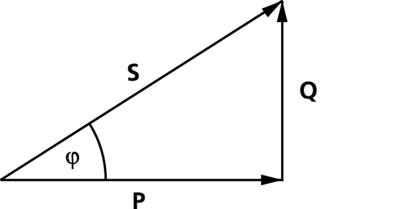
\includegraphics[width=0.5\textwidth]{Trojkat-mocy.png} % nombre del archivo
            \caption{Triángulo de potencia inductivo}
            \label{fig:triangulo_de_potencia} % etiqueta para referencias
        \end{figure}
    
    %%%Desarrollo%%%
    \indent
    \section{Desarrollo}

        \subsection{Procedimiento}

            Para esta experiencia se conectaron los instrumentos de medición junto con el variac y el inductor de la siguiente forma (Observar Figura: \ref{fig:circuito-inductor}). Luego se setió el variac a 120 V. Finalmente se procedió a la toma de mediciones de tensión, de corriente y la potencia usando el instrumental . 
            \begin{figure}[h!]
                \centering
                \begin{tikzpicture}
                    % Paths, nodes and wires:
                    \draw (22.5, -14.5) to[voltmeter] (22.5, -17.25);
                    \draw (24.25, -17.25) to[cute inductor, /tikz/circuitikz/bipoles/length=1.13cm, l={$L$}] (24.25, -15.75);
                    \draw (17.75, -14.5) to[ammeter] (20.25, -14.5);
                    \draw (20.25, -14.5) to[qpprobe] (21.75, -14.5);
                    \draw (21.75, -14.5) -- (22.5, -14.5);
                    \draw (17.75, -14.5) to[sinusoidal voltage source, l={$V_s$}] (17.75, -17.25);
                    \draw (22.5, -14.5) -- (24.25, -14.5);
                    \draw (17.75, -17.25) -- (24.25, -17.25);
                    \draw (24.25, -15.75) to[american resistor, /tikz/circuitikz/bipoles/length=0.924cm, l={$R_L$}] (24.25, -14.5);
                \end{tikzpicture}
                \caption{Circuito con fuente senoidal, amperímetro, voltímetro e inductor}
                \label{fig:circuito-inductor}
            \end{figure}

            Este procedimiento se realizó cuatro veces: a) Con el núcleo del inductor vacío. b) 
            Una barra de hierro parcialmente introducida en el núcleo. c) Con la barra de hierrototalmente introducida 
            en el núcleo. d) Con la barra de hierro laminado totalmente introducida 
            en el núcleo.

        \subsection{Mediciones}
            
            A continuación se presentan las mediciones tomadas en cada una de las cuatro instancias del experimento.

            \subsubsection{Núcleo vacío}

            \begin{table}[H]
                \centering
                \begin{tabular}{|c|c|c|c|}
                    \hline
                    $V_{rms} $[V] & $I_{rms} $[A] & $P $[W]  \\ \hline
                    120           & 1.175         & 29     \\ \hline
                \end{tabular}
                \caption{Mediciones con núcleo vacío}
                \label{tab:mediciones-nucleo-vacio}
            \end{table}

            \subsubsection{Núcleo de hierro parcialmente introducido}

            \begin{table}[H]
                \centering
                \begin{tabular}{|c|c|c|}
                    \hline
                    $V_{rms} $[V] & $I_{rms} $[A] & $P $[W] \\ \hline
                    122           & 0.6         & 16    \\ \hline
                \end{tabular}
                \caption{Mediciones con núcleo parcialmente introducido de hierro}
                \label{tab:mediciones-nucleo-parcialmente-introducido-hierro}
            \end{table}

            \subsubsection{Núcleo de hierro totalmente introducido}

            \begin{table}[H]
                \centering
                \begin{tabular}{|c|c|c|c|}
                    \hline
                    $V_{rms} $[V] & $I_{rms} $[A] & $P $[W] \\ \hline
                    124           & 0.25         & 12    \\ \hline
                \end{tabular}
                \caption{Mediciones con núcleo totalmente introducido de hierro}
                \label{tab:mediciones-nucleo-totalmente-introducido-hierro}
            \end{table}

            \subsubsection{Núcleo de hierro laminado totalmente introducido}

            \begin{table}[H]
                \centering
                \begin{tabular}{|c|c|c|c|}
                    \hline
                    $V_{rms} $[V] & $I_{rms} $[A] & $P $[W] \\ \hline
                    124           & 0.25         & 6    \\ \hline
                \end{tabular}
                \caption{Mediciones con núcleo totalmente introducido de hierro laminado}
                \label{tab:mediciones-nucleo-totalmente-introducido-hierro-laminado}
            \end{table}

        \subsection{Cálculos} \label{sec:Cálculos}

            \subsubsection*{Fórmulas utilizadas}

            Las magnitudes \textbf{medidas} de potencia activa $P$ (en watts), 
            tensión $V$ (en volts) y corriente $I$ (en amperes), se introducen en las siguientes
            expresiones para calcular las demás magnitudes de interés:

            \begin{enumerate}
                \item \textbf{Potencia aparente:}
                \[
                    |S| = |V| \cdot |I|
                \]
                donde $S$ se mide en volt–amperes (VA).

                \item \textbf{Potencia reactiva:}
                \[
                    Q = \sqrt{S^{2} - P^{2}}
                \]
                expresada en [VAR]. \par
                
                   La ecuación presentada aquí permite calcular el módulo de la potencia reactiva, pero como se dijo
                anteriormente esta puede tomar valores tanto positivos como negativos. En este trabajo práctico, 
                tomamos $Q=|Q|$ a sabiendas de que, dado que el único componente pasivo de nuestro circuito es inductivo, 
                la potencia reactiva será positiva también.

                \item \textbf{Factor de potencia:}
                \[
                    \cos \varphi = \frac{P}{S}
                \]

                \item \textbf{Ángulo de desfase:}
                \[
                    \varphi = \arccos\left( \frac{P}{S} \right)
                \]
                donde $\varphi$ se expresa en grados al convertir el resultado de 
                radianes:
                \[
                    \varphi \,[^\circ] = \arccos\left( \frac{P}{S} \right) \cdot 
                    \frac{180}{\pi}
                \]
            \end{enumerate}

                    Estas expresiones permiten representar el \textit{triángulo de potencias}, 
                    donde la potencia activa $P$ se ubica en el eje horizontal, la potencia 
                    reactiva $Q$ en el eje vertical, y la potencia aparente $S$ corresponde a 
                    la hipotenusa.\par

                Por otra parte, se calculó el valor de $L$ mediante la siguiente ecuación:

                \begin{equation*}
                    L = \frac{\sqrt{(I \cdot V)^2- P^2}}{\omega \cdot I^2} 
                \end{equation*}
                con $L$ la constante del inductor [H], $\omega$ la frecuencia [$\frac{rad}{seg}$], $V$ la tensión medida [V], $I$ la corriente medida [A] y $P$ la potencia reactiva medida [W]. \par
                
                    A continuación se presentan los triángulos de potencia de cada una de las configuraciones estudiadas, y en adición,
                    la configuración con núcleo totalmente introducido de hierro laminado. 

                    \subsubsection{Núcleo vacío}
                        Se obtuvieron los siguientes resultados:
                        \begin{itemize}
                            \item Potencia aparente (S): 141 VA
                            \item Potencia reactiva (Q): 137,98 VAR
                            \item Factor de potencia (cos $\phi$): 0,206
                            \item Ángulo de desfase $\phi$: 78,131°
                            \item Constante del inductor (L): 318,13 mH
                        \end{itemize}

                        \begin{figure}[H]
                            \centering
                            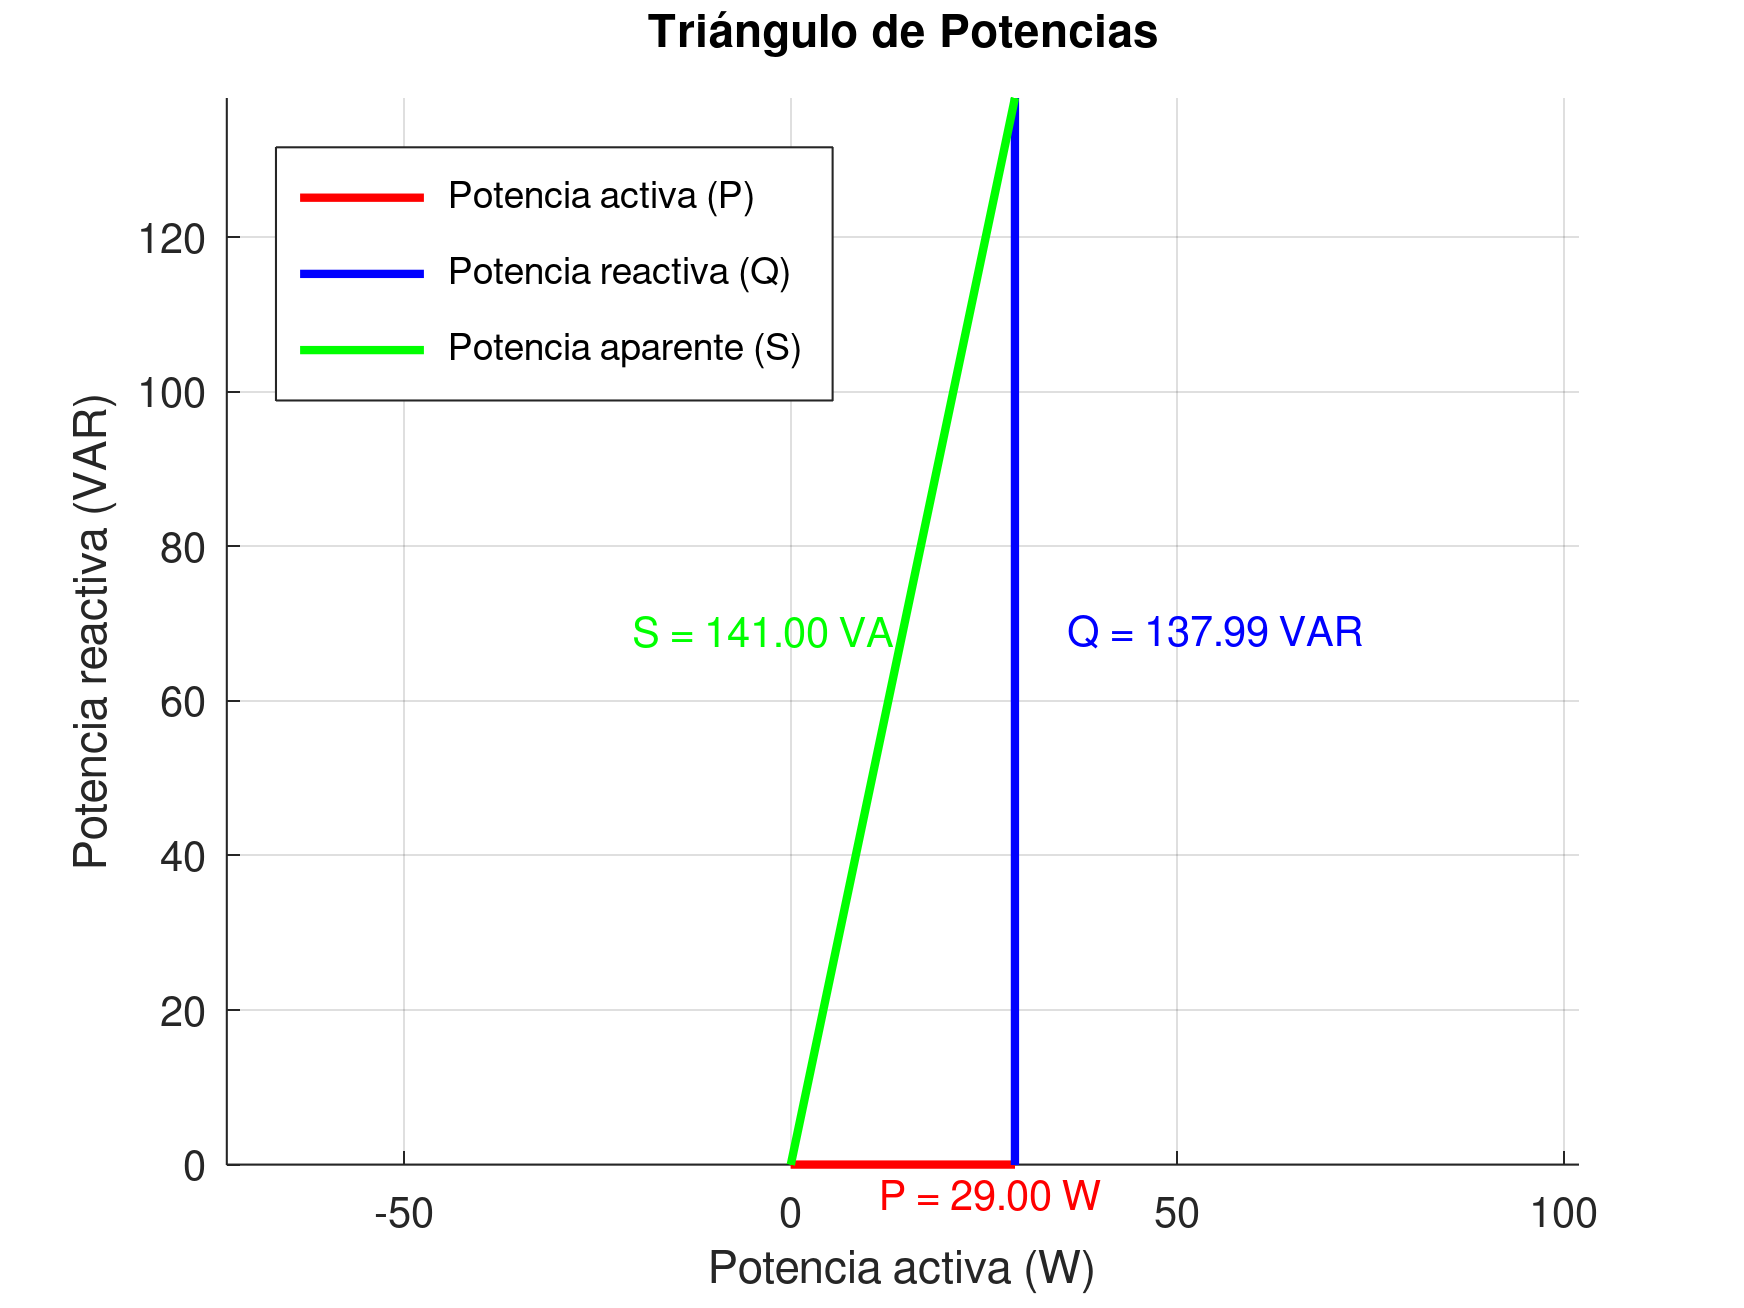
\includegraphics[width=0.8\textwidth]{graficoAire.png}
                            \caption{Triángulo de Potencias para el circuito con núcleo de aire.}
                            \label{fig:graficoAire}
                        \end{figure}
                    
                    \subsubsection{Núcleo de hierro parcialmente introducido}
                        
                        Se obtuvieron los siguientes resultados:
                        \begin{itemize}
                            \item Potencia aparente (S): 73,2 VA
                            \item Potencia reactiva (Q): 71,43 VAR
                            \item Factor de potencia (cos $\phi$): 0.218
                            \item Ángulo de desfase $\phi$: 73,37°
                            \item Constante del inductor (L): 631,58 mH
                        \end{itemize}

                        \begin{figure}[H]
                            \centering
                            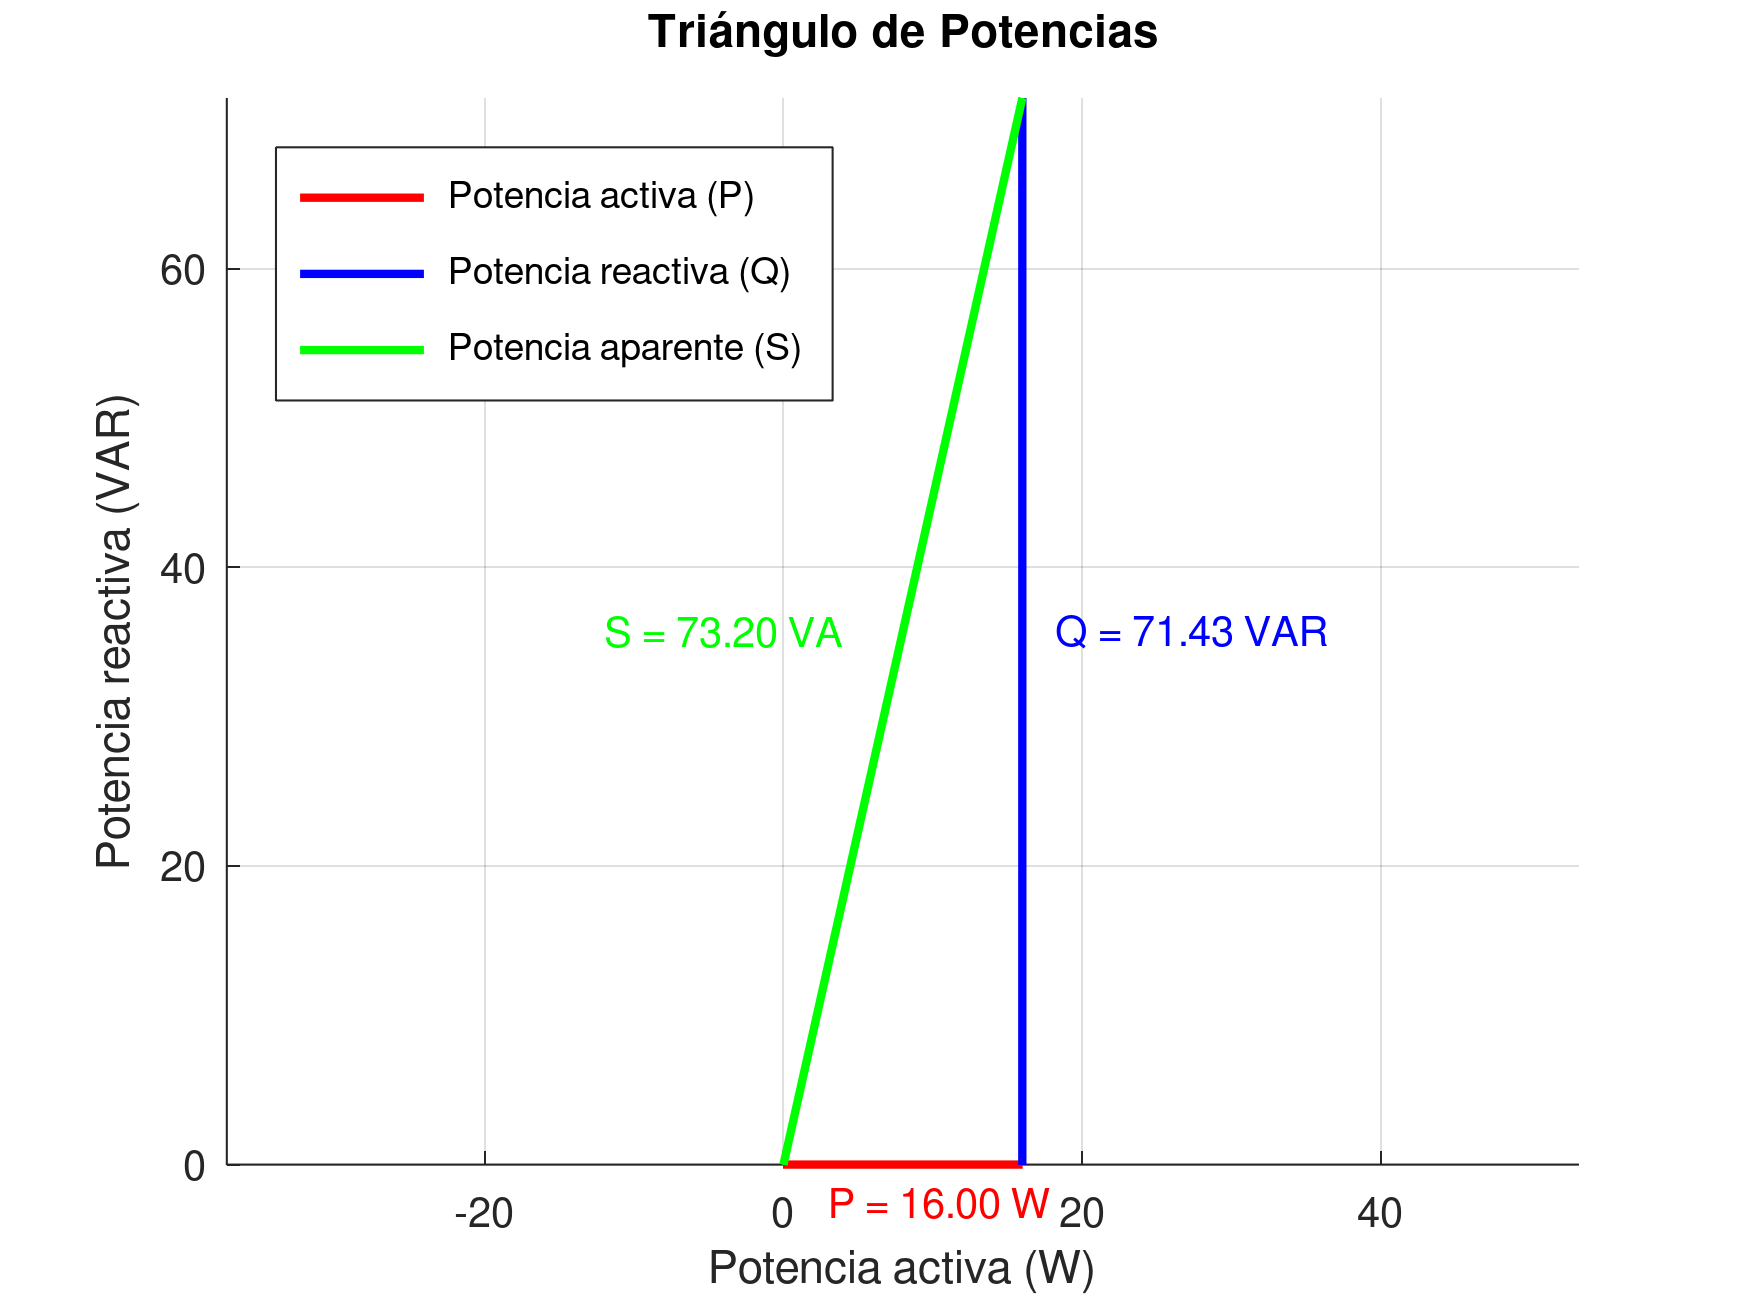
\includegraphics[width=0.8\textwidth]{graficoParcialHierro.png}
                            \caption{Triángulo de Potencias para el circuito con núcleo parcialmente introducido de hierro.}
                            \label{fig:graficoParcialHierro}
                        \end{figure}


                    \subsubsection{Núcleo de hierro totalmente introducido}

                        Se obtuvieron los siguientes resultados:
                        \begin{itemize}
                            \item Potencia aparente (S): 31.00 VA
                            \item Potencia reactiva (Q): 28.58 VAR
                            \item Factor de potencia (cos $\phi$): 0.387
                            \item Ángulo de desfase $\phi$: 67.23°
                            \item Constante del inductor (L): 1460 mH
                        \end{itemize}

                        \begin{figure}[H]
                            \centering
                            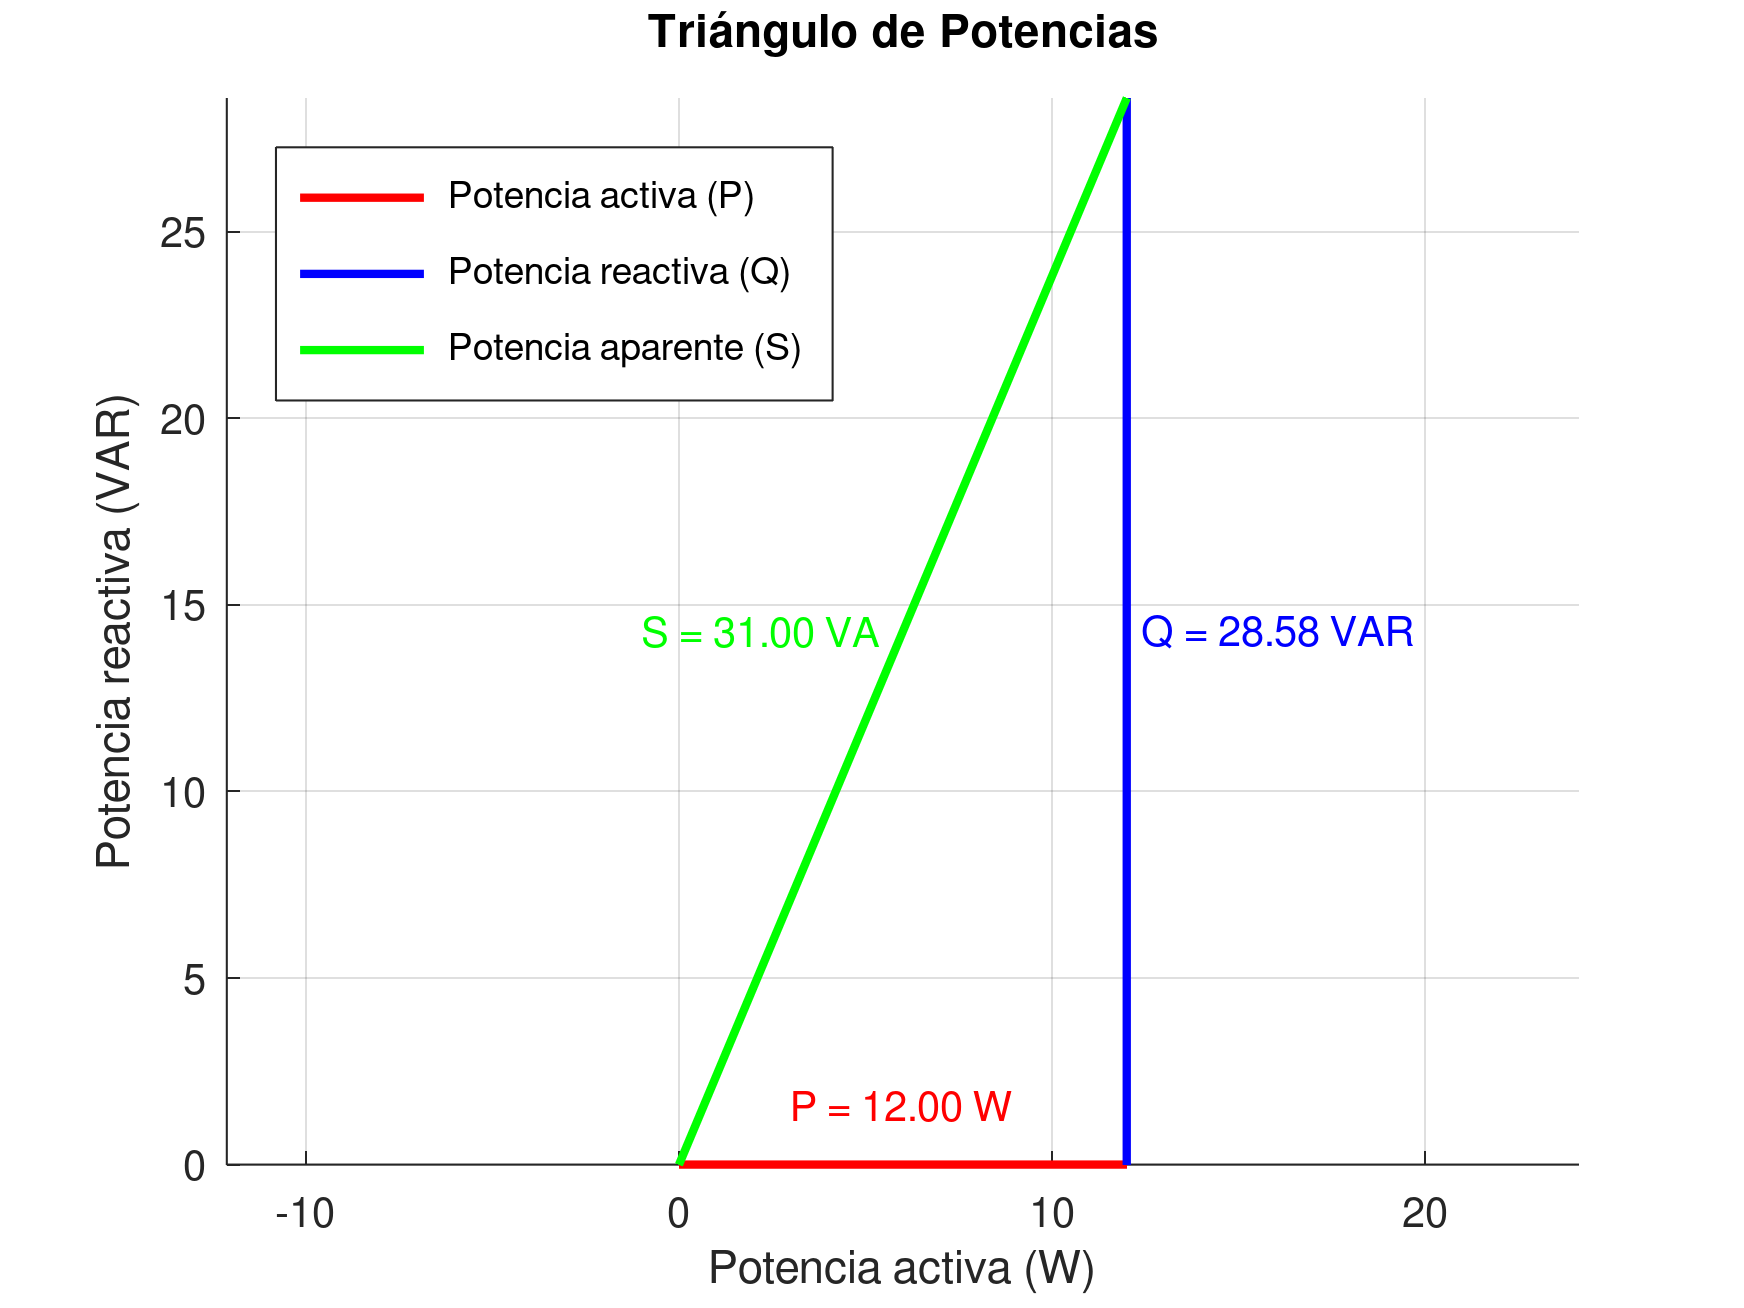
\includegraphics[width=0.8\textwidth]{graficoTotalHierro.png}
                            \caption{Triángulo de Potencias para el circuito con núcleo totalmente introducido de hierro.}
                            \label{fig:graficoTotalHierro}
                        \end{figure}


                     %   \subsubsection{Núcleo de hierro laminado parcialmente introducido}

                    %        Se obtuvieron los siguientes resultados:
                    %    \begin{itemize}
                   %         \item Potencia aparente (S): 70,15 VA
                  %          \item Potencia reactiva (Q): 63,43 VAR
                 %           \item Factor de potencia (cos $\phi$): 0,142
                %            \item Ángulo de desfase $\phi$: 81,80°
                  %          \item Constante del inductor (L): 668,47 mH
                 %       \end{itemize}

                %     \begin{figure}[H]
                    %        \centering
                %           \includegraphics[width=0.8\textwidth]{graficoParcialHierroLaminado.png}
                %           \caption{Triángulo de Potencias para el circuito con núcleo parcialmente introducido de hierro laminado.}
                %          \label{fig:graficoParcialHierroLaminado}
                %       \end{figure}
                    

                    \subsubsection{Núcleo de hierro laminado totalmente introducido}

                            Se obtuvieron los siguientes resultados:
                        \begin{itemize}
                            \item Potencia aparente (S): 31.00 VA
                            \item Potencia reactiva (Q): 30.41 VAR
                            \item Factor de potencia (cos $\phi$): 0.194
                            \item Ángulo de desfase $\phi$: 78.84°
                            \item Constante del inductor (L): 1550 mH
                        \end{itemize}

                        \begin{figure}[H]
                            \centering
                            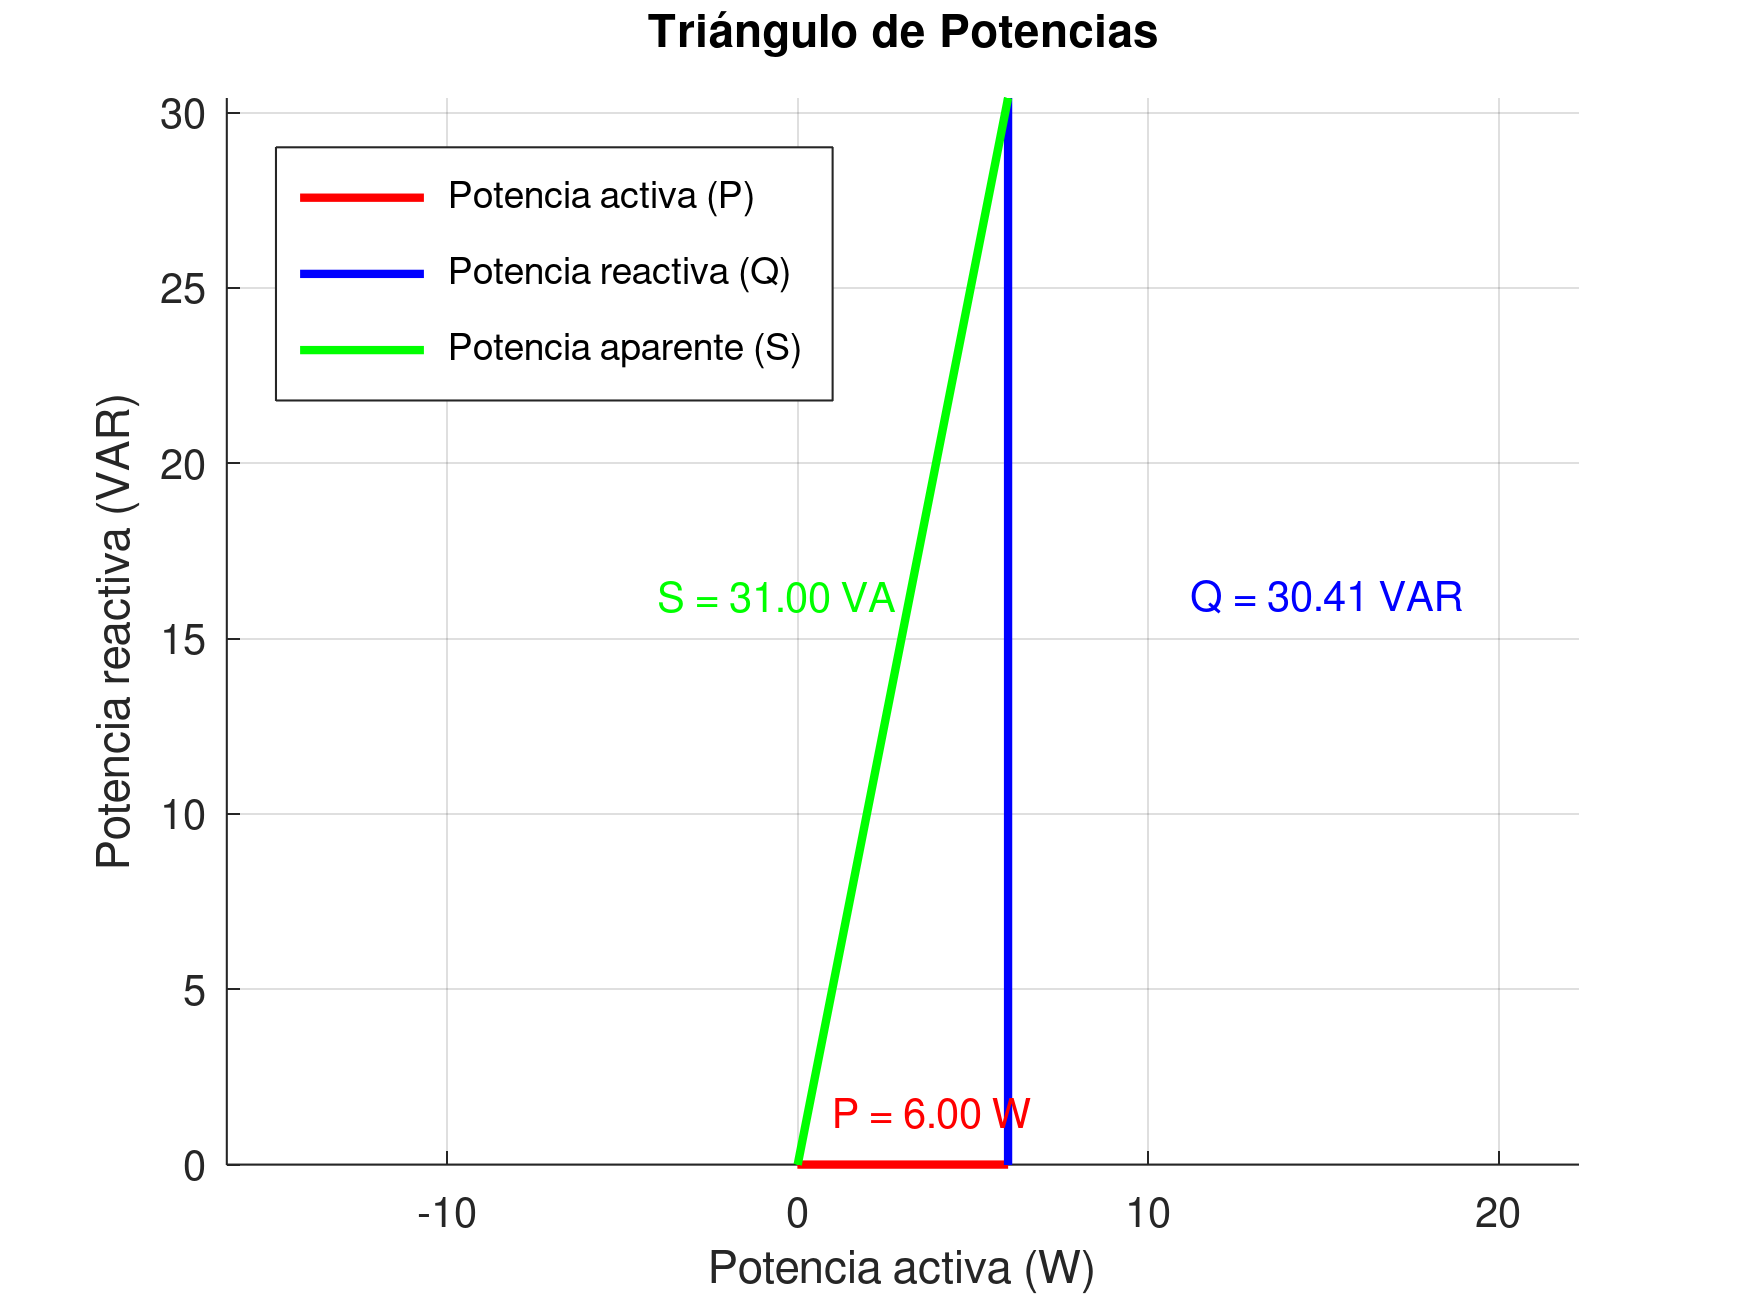
\includegraphics[width=0.8\textwidth]{graficoTotalHierroLaminado.png}
                            \caption{Triángulo de Potencias para el circuito con núcleo totalmente introducido de hierro laminado.}
                            \label{fig:graficoTotalHierroLaminado}
                        \end{figure}
            
                        
        \subsection{Análisis}
        
            Dado que se realizó el trabajo práctico empleando un núcleo de hierro y uno de hierro laminado, los valores
            de las inductancias obtenidas para una misma configuración con distintos núcleos son $L_{hierro} = 1460 mH$
            y $L_{hierroLaminado} = 1550 mH$, lo cual es esperable dado los materiales son muy similares.

            Además, se puede ver en la sección 2.3 que, dado que la inductancia de ambos núcleos es similar, la potencia
            reactiva (es decir, compleja) se ve principalmente afectada por la posición del núcleo en el inductor.
            \par También se puede notar en la tabla que la potencia activa disipada por el inductor se ve afectada por 
            la introducción de los núcleos. Obsérvese que el valor de la potencia activa disipada por el inductor una vez agregado
            parcialmente el núcleo de hierro desciende, luego es menor para el hierro introducido por compelto y aun menor para el
            hierro laminado.

            \begin{table}[h]
                \begin{tabular}{|p{5cm}|c|c|c|}
                \hline
                                                    &Potencia Activa [W]   & Potencia Aparente [VA] & Factor de potencia \\ \hline
                Sin núcleo                                &  29                      & 141 & 0,206    \\ \hline
                Núcleo de hierro parcialmente introducido     &      16                  & 73,2        & 0,218  \\ \hline           
                Núcleo de hierro totalmente introducido       &     12               & 31          & 0,387    \\ \hline           
                Núcleo de hierro laminado totalmente introducido & 6               & 31 & 0,194  \\ \hline
                \end{tabular}
                \caption{Mediciones indirectas de las variables de potencia afectadas por el inductor.}
                \label{tab:MedicionesIndirectas}
            \end{table}


            Luego, con el fin de cuantificar la imprecisión de las mediciones se decidió comparar la potencia activa
            medida de forma directa por el vatímetro con la potencia activa disipada por la resistencia interna del inductor
            (es decir, el único elemento pasivo que disipa potencia activa del circuito). Es decir, utilizamos la siguiente
             ecuación:
            \begin{equation}
               S_R = P = V_R \cdot I = I^2 \cdot R \cdot
             \end{equation}

            \begin{table}[h]
                \begin{tabular}{|p{5cm}|c|c|c|}
                \hline
                                                    & Medición Indirecta [W]   & Medición Directa [W] \\ \hline
                Sin núcleo                                        & 32,72                   & 29                        \\ \hline
                Núcleo de hierro parcialmente introducido            &       8,53        & 16                        \\ \hline
                Núcleo de hierro totalmente introducido             &      1,48          & 12                                 \\ \hline
                Núcleo de hierro laminado totalmente introducido   & 1,48               & 6              \\ \hline
                \end{tabular}
                \caption{Valores de la potencia activa para cada configuración obtenida de forma tanto directa como indirecta.}
                \label{tab:PotenciasActivas}
            \end{table}

            Se considera que la amplia disparidad entre los valores calculados y los obtenidos con el vatímetro se debe
            al margen de error del amperímetro de aguja para valores muy pequeños y muy grandes de corriente (relativos
            a la escala del amperímetro).

             
    %%%Conclusiones%%%
    \section{Conclusiones}
	En este trabajo, se observaron los cambios que hubo en la potencia disipada por la bobina y su resistencia interna en las distintas configuraciones. \par

Al introducir los distintos núcleos se observó una disminución de la corriente. Esto se debe a que la inductancia del inductor aumentó, incrementando la reactancia inductiva y, en consecuencia, la oposición al paso de la corriente. De este modo, la potencia activa se redujo gracias a la disminución de la corriente, tal como se esperaria acorde a lo estudiado en la materia. \par

Finalmente, se considera que para una mayor precisión en las mediciones se debe o trabajar con un amperímetro de menor escala, o bien aumentar la tensión de entrada con el propósito de aumentar la corriente. Esto permitiría trabajar con magnitudes de corriente que se acerquen al rango de mayor precisión del amperímetro. Esto taería el mismo efecto sobre la medición de la potencia activa, ya que aumentaría los valores de esta magnitud, llevándola a un rango donde el vatímetro tiene una mayor precisión.\par
    %%%Anexos%%%
    \section{Anexos}

\end{document}
